% This is samplepaper.tex, a sample chapter demonstrating the
% LLNCS macro package for Springer Computer Science proceedings;
% Version 2.20 of 2017/10/04
% TEMPLATE: https://www.springer.com/de/it-informatik/lncs/conference-proceedings-guidelines
%
\documentclass[runningheads]{llncs}
%
\usepackage{graphicx}
% Used for displaying a sample figure. If possible, figure files should
% be included in EPS format.
\usepackage{comment}
\usepackage{lettrine} % if you want the first letter to be \letterine{b}{igger}
%
% If you use the hyperref package, please uncomment the following line
% to display URLs in blue roman font according to Springer's eBook style:
% \renewcommand\UrlFont{\color{blue}\rmfamily}

\newcommand{\rom}[1]{(\uppercase\expandafter{\romannumeral #1\relax})}  % roman numbers with \rom{num}
\newcommand{\ber}[1]{(\lowercase\expandafter{#1\relax})} % (a)

\begin{document}
%
\title{Towards private Active Choreographies on public blockchain}
%
%\titlerunning{Abbreviated paper title}
% If the paper title is too long for the running head, you can set
% an abbreviated paper title here
%
\author{Henry Bergstroem\inst{1} \and
Jan Mensch\inst{1, 2}}
%
\authorrunning{F. Author et al.}
% First names are abbreviated in the running head.
% If there are more than two authors, 'et al.' is used.
%
\begin{comment}
\institute{Princeton University, Princeton NJ 08544, USA \and
Springer Heidelberg, Tiergartenstr. 17, 69121 Heidelberg, Germany
\email{lncs@springer.com}\\
\url{http://www.springer.com/gp/computer-science/lncs} \and
ABC Institute, Rupert-Karls-University Heidelberg, Heidelberg, Germany\\
\email{\{abc,lncs\}@uni-heidelberg.de}}
\end{comment}

\institute{Hasso-Plattner-Institut, Prof.-Dr.-Helmert-Straße 2-3, 14482 Potsdam, Germany 
\email{	bergstroem@uni-potsdam.de}
\and
University of Potsdam, Am Neuen Palais 10, 14469 Potsdam, Germany  \\
\email{jan.mensch@uni-potsdam.de}}

%
\maketitle              % typeset the header of the contribution
%
\begin{abstract}
\begin{comment}
BPMN, unstrusted, secred, hide participants, no central authority...
\textbf{The only thing that we leak is how many parties are participating in the entire business process}
honest-but-curious definition \cite{paverd2014modelling}
5 lines!

\end{comment}
\begin{comment}
motivation: Integrating business processes is good for the businesses
problem I: Businesses do not trust each other or a central authority
idea I: Ingo Weber solves this by doing it as active choreography on blockchain
problem II: Businesses do not want to share their data with each other
idea II: We solve it by providing our schema. 
evaluation: Implementation. We protect the logic of the business process, who is communicating and what is communicated, while still being enforcable and providing an unchaingable audit trail
\end{comment}


Integrating business processes was found to increase the performance of businesses. This collaboration is difficult if there is a lack of trust between the participating entities and between the entities and a third party. Active choreographies solve this problem, by making business processes enforceable. However they require that the business process and all exchanged messages are public. In this paper we provide an alternative approach towards active choreographies that keep the business logic, the exchanged messages and the identity of the entities exchanging messages secret, while still being enforceable. The schema can also be used to function as an audit trail. In addition to providing the conceptual background, we also make a prototype available, which executes a simple, predefined business process.


\keywords{Business Processes  \and Active Choreographies \and Privacy.}
\end{abstract}



\section{Introduction} \label{intro}

Blockchain \cite{nakamoto2008bitcoin}, invented by Saitoshi Nakamoto as a mean to solve the problem of double-spending in crypto-currencies, is a chain of digitally signed data (blocks). To sign a block, the hash of a block is calculated by applying a hash-function to the data of the block and the hash of the previous block. Nodes in the network have to "agree" on which block to include next, which is why there has to a consensus-mechanism (e.g. proof of work in the case of Bitcoin). Because appended blocks are computationally expensive to remove or alter and there is no central authority needed, blockchains can be used to serve as distributed, immutable data stores.

These capabilities (storing data immutably and having consent on a single state without the need of a  central authority) are greatly increased by networks like Ethereum. The technology enables developers to write smart contracts, Turing complete programs that are executed on the blockchain \cite{buterin2014next}.

Smart contracts are ideal for business process execution, since the entities collaborating with each other now have a single source of truth. Also since it is computationally expensive to retroactively change already submitted states, solutions that are based on smart contracts are ideal to serve as audit trails.

As shown in \cite{weber2016untrusted} there are ways to extend the use cases of business process execution and auditing to an untrusted environment, thus making it possible for entities to collaborate with each other that would usually not be  willing to do so. The execution of untrusted business processes is made possible by using Active Choreographies, which we will briefly discuss in section \ref{sec:rel_work}.

The goal of this paper is to extend \cite{weber2016untrusted}: We aim to make it possible to execute business processes in an untrusted environment and to enforce a business process without revealing its structure or purpose. Our approach also aims to keep secret what was communicated during the process execution and who was communicating, while still making sure that the predefined procedure is being followed by all participants. The schema also records an immutable audit trail that is only visible by entities that have a right to see it. 



\section{Background} \label{sec:background}

This section discusses the motivation, related work and the background which we took into account when designing our solution.


\subsection{Motivation} \label{sec:motivation}


\begin{figure}
    \centering
    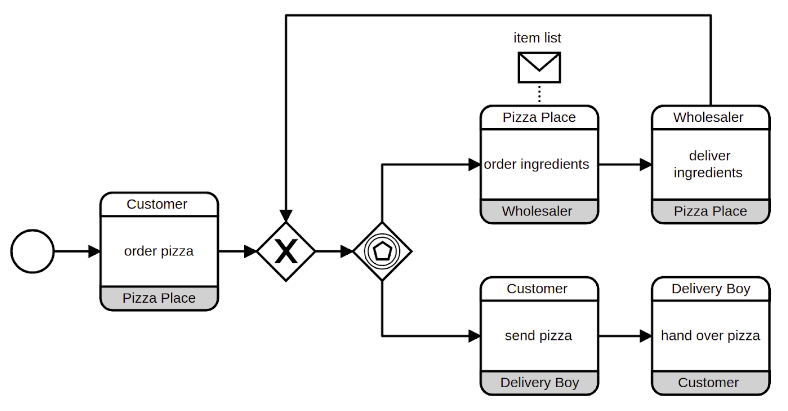
\includegraphics[scale=0.6]{bpmn.png}
    \caption{A simple choreography diagram}
    \label{fig:simple_bpmn}
\end{figure}

\textbf{taken from the paper form ingo weber!}
Integrating business processes has been found to have a positive impact on the operational and business performance \cite{flynn2010impact,narayanan2011antecedents}. However a lack of trust between business partners is hindering such progress \cite{panayides2009impact}. By providing a solution that needs neither trust between participants, nor in any central authority and keeps the business done secret, we hope to further increase collaboration between businesses. 

\textbf{mention business process mining?} \cite{van2007business}



Our motivation can be summarized in the following statements: \ber{a} There are several parties which want to collaborate. These parties have \ber{b} neither trust in each other nor \ber{c} trust in any third party. They \ber{d} furthermore want to keep their business process secret, \ber{e} hide with whom they are collaborating and \ber{f} hide what messages are exchanged during the collaboration. Since the parties distrust each other they also \ber{g} only want to share messages with the entities that have to see them and keep them secret from the others.

\begin{comment}
\begin{itemize}
    \item there are several parties who want to collaborate 
    \item parties have no trust in each other 
    \item parties have no trust in a third party
    \item parties have strong interest in keeping things secret
\end{itemize}
\end{comment}




Throughout this publication we will try to present our thoughts in more concrete fashion by applying them to the example shown in figure \ref{fig:simple_bpmn}. Here the parties are \ber{a} collaborating without trust (\ber{b} and \ber{c}). They also have an urge to keep as much as possible about their collaboration secret (\ber{d}, \ber{e} and \ber{f}). An example for \ber{g} would be that the \textit{Delivery Boy} should not know anything about the collaboration between \textit{Wholesaler} and \textit{Pizza Place}, even though he is part of the overall business process. 

\begin{comment}
It displays the process of ordering, making and delivering pizza. In the process the \textit{Pizza Place} can decide weather to deliver straight away, using the \textit{Delivery Boy} as a middle man, or if it has order ingredients at the \textit{Wholesaler}. We chose a choreography diagram to display the process in order to emphasis the collaboration between the participants. Please keep in mind that in reality business processes might be much more complex and may involve many more participants. The example is kept simple on purpose and only serves as an illustration for our approach. 
\end{comment}




\subsection{Related work} \label{sec:rel_work}




\bigbreak
\textbf{Explain the levels of secrecy}. 
\begin{itemize}
    \item Model-layer
    \item Communication-layer
    \item Content-layer
\end{itemize}




\bigbreak
\textbf{Active Choreography}. In \cite{weber2016untrusted} Weber et al. explain how a business process can be enforced in an environment where the participants do not trust each other. By using a smart contract, acting as an active mediator between participants. The term active mediator implies that the component is able to accept or reject messages and makes sure that the business process is executed as specified. With the help of this and other components they are able to \rom{1} execute collaborative processes over a network of untrusted nodes, \rom{2} enforce that only conforming messages can trigger state-changes, \rom{3} payments and escrows can be coded in the business process and \rom{4} an immutable audit trail keeps track of all transaction. Furthermore none of the participants in the business process has to organize the collaboration, which is what differentiates a choreography from a orchestration \cite{some_source}. The approach introduced in \cite{weber2016untrusted} is different from ours in the sense that in their implementation the business process is included in the smart contract, which makes it public. It displays which participants are collaborating with each other, how they are doing it and what messages are exchanged. There is no point in trying to encrypt messages that trigger a state-change, since these messages have to be processed with the smart contract and all calculations done on the smart contract are public. We aim to change this and try to hide what the business process, who is participating in it and what messages are exchanged, while still providing that \rom{1}, \rom{2} and \rom{4} hold. \textbf{Explain why \rom{3} does not hold???}

For the scope of this publication we define an active choreography as a decentralized collaboration between nodes where no node has to orchestrate the process and the choreography is set up in a way that invalid state-changes can be rejected, thus making sure that the predefined procedure is always followed. 




\bigbreak
\textbf{Privacy Enhancing Technologies on the Blockchain}.
\begin{itemize}
    % https://blog.ethereum.org/2016/01/15/privacy-on-the-blockchain/
    \item private blockchain (why is this more private? What kinds are there?)
    \item ring signatures
    \item homomorphic encryption
    \item zero knowledge proofs -> zero cash
    \item partiy.io. Also does secret messages. Has a private contract in the smart contract. We are better, because we can hide content from each other (concept of circles). Do a picture with where you are comparing the architecture (siehe mein colledge block)
\end{itemize}

This section aims to give a quick overview of technologies and applications that we took into consideration when implementing this prototype. We also indicated which layer might be influenced by the respective approach. 

One of them is \textit{obfuscation}, which we could use to hide the model (our business process). This is a technology that "aims to make a computer program 'unintelligible' while preserving its functionality" \cite{garg2016candidate}. If we could make use of it, it might be possible to hide the functionality of our business
process on a public blockchain in "plain sight". Since it was shown in \cite{barak2001possibility,barak2012possibility} that there were a set of functions that are impossible to obfuscate, the idea of indistinguishable obfuscation was
introduced. This is a weaker constraint, guaranteeing that it is impossible to distinguish two equivalent programs have
been obfuscated. These ideas seem to be very powerful, but come with a big drawback: According to \cite{banescu2015idea}, to even generate an obfuscation of a 2-bit multiplication circuit would take about $10^{27}$ years on a 2,6 GHz CPU. Obfuscation at its current state is thus not feasible. 

Another technology aiming to increase privacy in distributed applications is \textit{secure multi-party computation (SMPC)} \cite{orlandi2011multiparty}. With SMPC, there are are multiple parties involved in computing the output of a function, without having to trust each other. They thus need a protocol that makes sure that the output is correct and that cheating participants will not be able to learn anything about the input of the honest parties. An algorithm with these properties could provide us with a way to compute the current state of our business logic without letting some parties know the input that triggered that state (content-layer). \textbf{Inefficient \textbf{SOURCE?}. Why did we not use this? -> model layer}

A technology already in use in blockchain applications are zero-knowledge Succinct Non-interactive ARguments of Knowledge (zk-SNARKs). Applications using this are e.g. Zerocoin which aims to provide fully anonymous currency transactions \cite{miers2013zerocoin}. zk-SNARKS provide the possibility to have an untrusted prover very a statement made by a different party without that party having to reveal their statement \cite{ben2013snarks}. It furthermore does so in a non-interactive manner. If we think of our model as a state-machine, we might use zk-SNARKs to prove that a state-change is valid without actually communicating the respective message(s) (message- and content-layer). However we do not see how we could use zk-SNARKs to keep the model-layer secret. This might be a field of future work and if feasible, might be a better solution than the one we are providing right now. 




\section{out of scope things}
I will at some point mention some things that are out of scope of this publication. How to exchange symmetric keys using asymmetric key encryption (compare OpenPGP and give broken down example of how that works. Mention that we did not implement it, to focus on the important stuff). How to agree on who should send it. We could also just have one node always send it to the chain. That would work, since an outsider would not know what is going on (no extra information, like who is the originator of the message). But since the participants do not trust each other using a random node to send the message is better. Selecting a random node can be done by using a distributed consensus protocol (like electing a leader in distributed databases. Just mention a possible algorithmn here).   



\section{some section}


\subsection{Tradition Solution}
parties have to trust each other 

there is a third party involved

there is one party that controllers everything (a very strong party, e.g. Amazon)


\subsection{Alternative solution with Blockchain Technology}
here we explain how active choreographers work and cite from the paper again \cite{weber2016untrusted}. Also now we have to show that if we choose an active choreography as a solution, there are two possible paths to take: 

\begin{enumerate}
    \item make everything public. We don`t want this to happen. This would be the approach described in \cite{weber2016untrusted}.
    \item have a private blockchain. For that we would have to trust the party, which is hosting that private chain. We don`t like this solution, because we are paranoid. 
    \item use cryptography to keep it hidden in plain sight (our approach).
\end{enumerate}

\section{Approach}
\subsection{Assumptions}
The following assumptions are made: 
\begin{itemize}
    \item the blockchain is public
    \item everyone can see what is posted on the blockchain
    \item an adversary does not track the traffic from individual participants from and to the blockchain. Therefore if the name of sender of a message is not stored in plain text on the chain, nobody knows who send the message.
    \item the participants of a business process (BP) do not trust each other, but would like to cooperate with each other
    \item it is possible to express any BP with a program and this program can enforce the corresponding business process
    \item it is possible for a program on the chain to notify a party (avoid busy-wait) 
    \item This program can be viewed as a state-machine
     \item an entity that is part of a message exchange is allowed to see that message in the audit trail
     \item All nodes/entities are always online and node failure does not happen. This is unrealistic, but it is kept out of scope on purpose, to be able to focus on the privacy stuff.
     \item Clients are honest but curious: Everyone follows protocol, no one can forget anything they learned. Whatever info they can get they will get. Secure if a party only gets as much knowledge as they should (Defined in \cite{xiong2011cloudseal} \cite{paverd2014modelling})
\end{itemize}

\subsection{Ideal solution}
The ideal solution would look something like this: 
\begin{itemize}
    \item process uses a public blockchain
    \item A participant can enable a third trusted party to view all communication (audit trail) if (and only if!) one of the participants of that communication grants that third party permission to do so. Example: A is a supplier, B a seller, C the logistics guy, sending stuff from A to B, E the buyer, who buys stuff from B and F the logistics guy sending stuff from B to E. Something went wrong when ordering the supplies. A is unhappy with this and calls a lawyer. A can provide the lawyer with the audit trail of the communication he was involved in (e.g. between A and B, A and C and between A, B and C) but he can not give the lawyer any other communication, since he himself can not see that.
    \item parties agree on a process and that process has to be executed exactly as specified
    \item the parties only have to communicate via the blockchain
    \item execution of a BP is cheap (cost of gas on Ethereum)
    \item an observer, who read everything on the public blockchain that is used as a mediator between the parties can not know derive any conclusion about how the business logic looks like (logic), who send what messages when (message) and what messages where send (content).
\end{itemize}


\subsection{Where should the logic of the business process be kept?}

As mentioned before we try to enforce a business process (BP) with an active choreography while still keeping the content, communication and (in part) the model secret. Since we are in favor of using a public blockchain, we can consider all logic (model layer) and all communication that is done with a smart contract running on such a blockchain as public. We could encrypt the messages exchanged between smart contact and the participants of the Business Process. This would keep the content and possibly the communication secret, but if we keep the logic of the BP public that would be of no use. A simple example to illustrate this point:

\begin{figure}
    \centering
    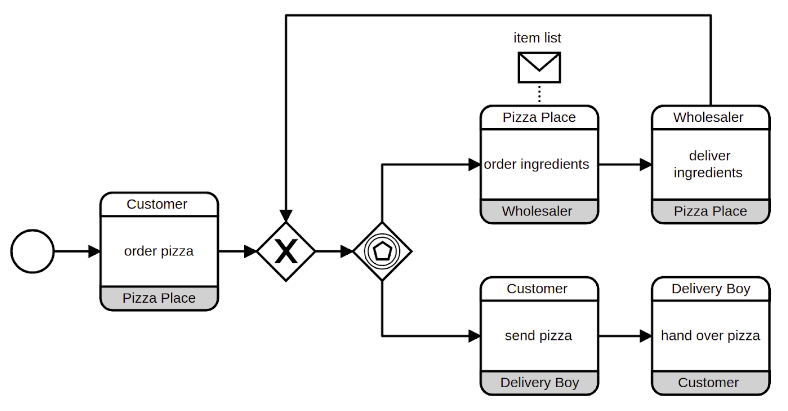
\includegraphics[scale=0.6]{bpmn.png}
    \caption{A simple BPMN}
    \label{fig:BPmn}
\end{figure}

If we implement the BP shown in \ref{fig:BPmn} as an active choreography and upload it to a public blockchain there is no point in trying to keep any of the communication secret. What do we mean by that? Let`s assume an observer tracks all communication done with the active choreography, but has no understanding what is being communicated and who is sending which messages. The observer does not need this information to be able to understand the communication. She can just watch the state-changes in the BP. If, for example, the state changes to \textit{ordered pizza}, the observer knows that a customer just ordered a pizza. If it then changes to \textit{order ingredients}, the observer understands that \textit{Pizza Place} does not have enough ingredients to process that order. Even if we try our best to keep content and communication secret, if we keep the state of the BP public, an outsider might be able to understand who is communicating and what is being communicated. The only thing we might be able to keep secret are mere details about the communication. For this reason we propose to keep the model off-chain. 


\subsection{Implementing an active choreography off-chain}

An active choreography will make sure that a business process is executed as defined. Any attempt by a participant to evoke an illegal state-change will be rejected, since the business process knows what state-changes are legal and under what conditions they are carried out. This approach is no longer possible, if the active choreography is not aware of the business logic. Instead the clients would have to agree on what BP to execute and in which state they are. To keep a record of what business process is executed, the clients could share a hash of that BP (or rather the code representing it) and store it on the blockchain. 

If a client now wants to execute a state-change in the BP, there should be a consensus among all clients that this state change is legal. If we use a "normal" consensus protocol this would not keep a client from cheating, since the choreography has no knowledge of a consensus reached between the clients. An example: \textit{Customer} wants to order a Margarita pizza. For that he would like to do trigger a state change. For that he drafts the message \textit{Order Margarita for 5 EUR}. If we have a consensus protocol, e.g. based on voting the other clients could now accept or reject that message and with it the state-change. Let`s assume they accept it. \textit{Customer} now sends the message \textit{Order Margarita for 1 EUR} to the active choreography, which, with a client-based consensus protocol, has no way of rejecting this message as illegal. 

To prevent this from happening a feasible consensus protocol might look like \ref{fig:simple}, with $S_x$ being the secret key of each participant. In our example \textit{customer} drafts the message \textit{Order Margarita for 5 EUR} and encrypts it with his secret key $S_c$. The message is then send of to all other participants. Each of whom encrypt it with their secret key. 


\begin{figure}
    \centering
    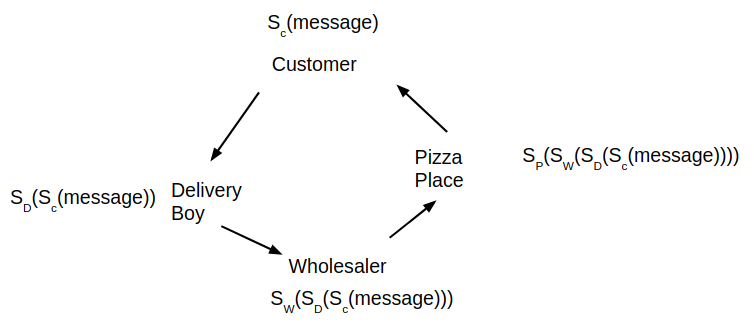
\includegraphics[scale=0.6]{simple_consensus.png}
    \caption{The simple version of the consensus protocol}
    \label{fig:simple}
\end{figure}


At the end the four times encrypted message reaches \textit{customer} again. He than sends it to the active choreography together with the order they were encrypted in and the actual message. The message might look something like this \textit{cipher, message, [C, D, W, P]}. The active choreography is in possession of all public keys. It applies them in order to the cipher and compares the result with the message. If they are the same and all public keys were applied to the message it knows that there was a consensus between all clients. 

What happens in the case of a disagreement? Let`s assume that the actual cost of the Margarita pizza is 6 EUR, not 5 EUR. The \textit{pizza place} on receiving and encrypting  $S_W(S_D(S_C(message)))$ will simply not encrypt it with its own private key. \textit{Customer} has no way to still do a state-change, because the active choreography will reject the message, if it was not encrypted by all participants. 

What happens if \textit{customer} or any other participant tries to cheat? Customer will receive $S_P(S_W(S_D(S_C(message))))$ and can encrypt it. If he replaces \textit{message} with something else, he will fail to encrypt it again, since he is not in possession of the other secret keys. The active choreography will therefore reject the message. The same is true for all other participants. 


\subsection{Advancing the idea of the simple consensus protocol}

There are multiple drawbacks from the simple consensus protocol displayed in -\ref{fig:simple}: 

\begin{enumerate}
    \item In order for the active choreography to be able to reject an invalid message, we have to provide it with the original message. We would like to avoid that to keep the content of the message secret (content layer).
    \item Every participant of the BP will know all messages exchanged, even messages which do not affect him. 
    \item An observer will always know who the originator of the message was, since it is always the first client in the provided order. In our example the order was \textit{[C, D, W, P]}, which in this protocol, makes it obvious that this is a message from the owner of the C key-pair.
    \item A client which goes rouge could always block further progress in the BP, by no longer encrypting messages.
\end{enumerate}

The first and the second drawback can be by using symmetric keys to encrypt messages per "interest group". An interest group (we call them "circle") is the group of clients which are allowed to read a message, because they participate in the part of the business process that this particular message is relevant for. An example: 

\begin{figure}
    \centering
    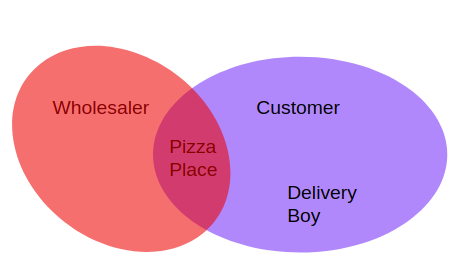
\includegraphics[scale=0.6]{cicles.png}
    \caption{The circles in the example BPMN}
    \label{fig:circle}
\end{figure}


As shown in \ref{fig:circle}, \textit{customer} is in a circle with \textit{pizza place} and \textit{delivery boy}. \textit{wholesaler} is not in that group. This is because \textit{wholesaler} should not know what e.g. \textit{customer} and \textit{delivery boy} are communicating. To enforce the circles, both groups will exchange symmetric keys, prior to the execution of the BP. This symmetric key exchange can be done safely, since they participants can exchange symmetric keys using asymmetric key encryption (similar to OpenPGP  \textbf{citation needed!}). To exchange messages, the clients will now first encrypt them with the symmetric key of their circle and then send it on to the other clients (compare \ref{fig:complex}). A client which is in a circle will be able to encrypt the message. All other clients will not be able to read it. Like before one client from the group will have to send the encrypted message and the order of the applied keys to the active choreography. The example from above will now look as follows: \textit{cipher1, cipher2, [C, D, W, P]}, with \textit{cipher1 =} $S_P(S_W(S_D(S_C(cipher2))))$, $cipher2 = Sym_{blue}(message)$, \textit{message = Order Margarita for 5 EUR} ($Sym_{blue}$ is the symmetric key of the blue circle).

Like before the smart contract is now able to reject any message, which was send without the consent of all clients participating in the BP. Also, since a message has to be signed by all clients, not only by the clients of the relevant circle, an outsider will not be able to know who is collaborating with whom. The total number of circles, the size and the members of any circle will remain secret. 

To solve the third drawback (observer is able to determine the originator of a message), we can propose the the following schema, depicted in \ref{fig:complex}. Among all clients there one client will be chosen, sending the above message for someone else. This participant could either be chosen randomly for each message or once for the entire BP. The former approach would require less trust among all clients, the latter would make it possible to only "register" one communicator at the active choreography and thus keeping secret who is participating in the BP (communication layer). \ref{fig:complex} shows how the example from above could look like in the complex version of the consensus protocol.

\begin{figure}
    \centering
    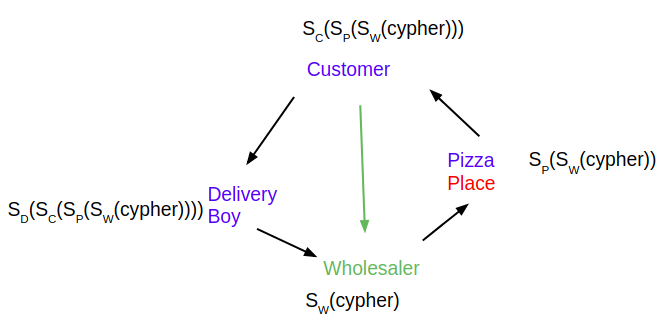
\includegraphics[scale=0.6]{complex.png}
    \caption{The complex version of the consensus protocol}
    \label{fig:complex}
\end{figure}


We assigned each client a color, depending on their circle membership. We assigned green to \textit{wholesaler} to symbolize that this client will send the message to the chain, even though the \textit{customer} is still the originator of the message. The schema works as follows: The originator of the message (\textit{customer}) will send cipher2 to the client responsible for communicating with the active choreography (\textit{wholesaler}, exchange of cipher2 is the green arrow). That client will than send it on to the next client, who will send it on to the next... Like before all clients will encrypt it with their secret key. The message that \textit{wholesaler} will send to the active choreography will be \textit{cipher1, cipher2, [W, P, C, D]}, with \textit{cipher1 =} $S_D(S_C(S_P(S_W(cipher2))))$, $cipher2 = Sym_{blue}(message)$, \textit{message = Order Margarita for 5 EUR}. 

What happens if the client responsible to communicate with the active choreography tries to cheat? After all, if he is part of the same circle as the originator of the message, he can read cipher2. Still this should not matter, since all clients have to encrypt the message. If \textit{wholesaler} cheats, \textit{customer} will detect that and refuse to encrypt the message. Furthermore a message will always be rejected if not encrypted by all members of the BP.



\begin{comment}

\textbf{keep logic secret:} The program $P$, matching the BP should be kept on client side. Since we are just communicating via the Blockchain, the communication of how this process looks like should be done on-chain. For that $P$ should only be stored in encrypted form on the chain. If someone tries to cheat and executes a different program, this will be obvious later, since a record of the actual program (or a hash of it) is kept on-chain. 

\textbf{keep message and content secret:} It should be possible for messages (and logic) to be seen only by parties that are involved in processing those messages. Therefore we need some sort of encrypted "broadcast" of a message within a group. Some of the groups from the example above could be as following (just an example): $G_1 = \{A,B\}$, $G_2 = \{A,C\}$, $G_3 = \{A, B, C\}$, $G_4 = \{E, B, F\}$. So within $G_1$, $G_2$, $G_3$ and $G_4$ we should be able to exchange messages without the other participants (or an outsider) realizing who send a message (secret message) and what was send (secret content). A proposed solution to establish this "encrypted broadcast" for $G_3$ (or any other group): 

\begin{itemize}
    \item A, B, C each generate a key pair. Key pair for A is denoted as public key: $pk_A$, private/secret key $sk_A$. They post it on the chain. The chain now contains $pk_A$, $pk_B$, $pk_C$.
    \item One of the group (lets say A) is chosen as a master. He is kicking off the process
    \item A is now generating a symmetric key $S$
    \item A is posting $pk_B(S)$ (S encrypted by public key of A), $pk_C(S)$  to the chain. B and C now take those values and are thus in position of $S$. Nobody else besides of A, B and C knows $S$
    \item A will post $pk_A(hash(S))$. Everyone can check, if the hash matches up with his/her version of $S$. If it does not, we know that Something went wrong.
    \item If B wants to broadcast in $G_3$ now he is posting $S(sk_B(message), B)$ (his name encrypted with $S$ and the encrypted message encrypted with $S$. This way we know that the message is from B. We do not have to check if the message is from A or C, since it says that it is from B. Nobody else knows that it is from B, since it is also encoded by $S$. Also nobody knows the content.
\end{itemize}

This process is distributed (no third party needed) and requires no trust. Also the blockchain is only used as storage and there are no cryptographic operations done on-chain, so the operations are (hopefully) affordable.

\textbf{further thoughts:} Since we can view the PB as a state-machine, every state change must be posted to the chain. We can do this with the process described above. State changes have to be reflected on client side. 

\textbf{questions}: Things I am not sure about, that I would like to talk about
\begin{itemize}
    \item Do we need some sort of consensus protocol to make sure that all clients are in the same state?
    \item How do we convert a BPM into code? Are the assumptions correct?
    \item  Is the ideal solution really the ideal solution? 
    \item Does the encryption idea make any sens?
    \item Is there a better way to enforce that the correct program is being executed on client side?
\end{itemize}


\end{comment}


\section{Architecture Alternatives}
We have discussed a range of different alternatives of how the architecture can look like. Each architecture has its advantages and disadvantages.

\textbf{Where to put the code associated with the business logic?}
The blockchain acts like the source of truth for the actors. One main question is what is best to keep on the blockchain and what is better off. To maximize uniforminess between the actors it would make sense to have all logic on the blockchain. The obvious downside with the blockchain is that it is expensive to use and that everything is public. Depending on the business choreography and its priorities the better choice might be to leave parts of the business logic off-chain. The following table highlight the pros and cons about having the code on or off chain.

\begin{table*}[t]
  \centering
  \begin{tabular}{p{6cm}p{6cm}}
  \hline
    \textbf{On-Chain} & \textbf{off-Chain}\\
    \hline \hline
    
 expensive & cheap \\
     harder to scale & easier to scale \\
     more transparent & more secret \\
     enforceable & not directly enforceable \\

\hline
  \end{tabular}
  \caption{Explain table here}
  \label{tab:1}
\end{table*}


\subsubsection{How to make enforce an off-chain choreography}

If we decide to have the code code off-chain, to ensure that the business logic is kept secret, the question is how to ensure that a agreed upon business process will still be executed as specified. Since the smart contract in that case would only save the current state of the business process, it would have no way of knowing which state change would be legal or illegal to execute next.

An example: Alice $A$, Bob $B$ and evil Eve $E$ would like to participate in a business process. $E$ intends to be cheating (meaning not executing the business process in the pre-defined order). All three parties agree on a business process that should be executed. This business process is compiled to executable code. To consolidate this, they save a hash of this code on-chain. All parties now start to execute the business process. There are therefore state-changes to the business process. This state changes are reflected on-chain, without any outsider being aware of the underlying business process. The smart contract thus acts as an interface between the clients and the blockchain, which here plays the role of an audit trail, not an active choreography. If $E$ now sends an illegal state change to be recorded in the audit trail, the smart contract has no way of rejecting that, since it itself does not know if the proposed state change is legal or illegal.

A technique to avoid this is introduced by parity \footnote{https://wiki.parity.io/Private-Transactions}: In their implementation before a client can communicate with the blockchain, it has to validate its communication with a validator. \textit{How does the chain know that the validator has validated the client? Assumption: It will check the signature of the client and the validator and know that this validator is responsible for that client.}. To avoid all this overhead and to make communication more private, we propose to use a ring signature. Ring signatures were first introduced in 2001 by Rivest et al. and make it possible to specify a group of possible signers without giving away who the actual author of a signed message is \ref{rivest2001leak}. Ring signatures are already used in combination with blockchain technology, among others the CrypoNote protocol used in the Monero network \ref{van2013cryptonote}. In the protocol, a participant can not know from who or to who he or she is sending money or is receiving money from, only that the sender or receiver is part of a one-time ring signature.



We propose that there exists exactly one ring, which includes all participants (regardless of their circle). If a participant now wants to have a state-change confirmed he/she has it signed by all other participants in the ring. A participant who is in the same circle as the sender can read the message. If he she disagrees with the content of the message (the state-change) he can communicate this back to the sender and prevent the state change. Since the smart contract can check if the message was signed with the ring signature $E$ has no way of submitting an invalid state-change. We now moved from an audit trail to an active choreography. 

There is still an obvious flaw in the proposed implementation: How do we prevent $E$ from halting any state change at any moment? She could just interrupt the continuity of the business process. So far we do not have any good answer to this. We could hope that it is still in the best interest of $E$ that the business process is fully executed and she therefore would not want to interrupt it. A more technical option would be to have the clients generate random messages to confuse $E$, so that it at least would be very hard for her to halt the business process at a certain state. However this is just a suggestion and topic to further research.


How can a client prove to the chain that the proposed state-change is legal?
zero-knowledge?
confirmation of other clients
\bibliographystyle{splncs04} % BibTeX users should specify bibliography style 'splncs04'.
\bibliography{refs} % Entries are in the "refs.bib" file


\end{document}
